\section{Architettura}

L'architettura del prodotto è suddivisa in:
	\begin{itemize}
	  	\item \textbf{gateway};
	  	\item \textbf{piattaforma Apache Kafka};
	  	\item \textbf{data collector};
	  	\item \textbf{database PostgreSQL e Timeseries};
	  	\item \textbf{API REST};
	  	\item \textbf{bot Telegram};
	  	\item \textbf{web application}.    
	\end{itemize} 

	\begin{figure}[H]
		\centering
		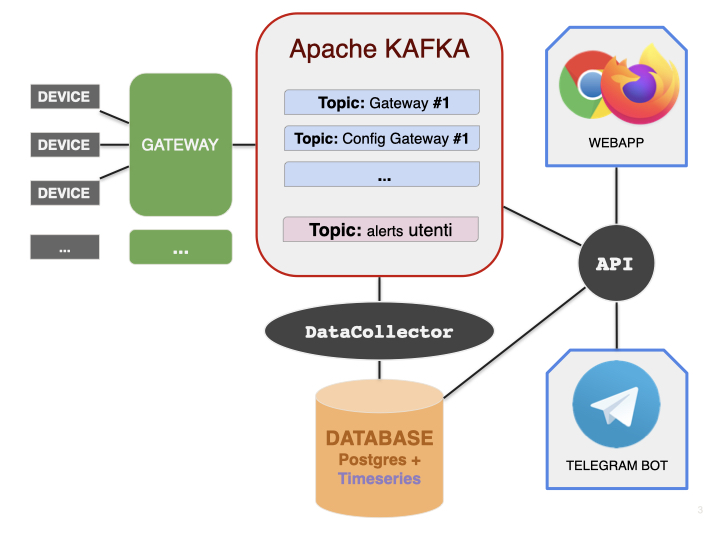
\includegraphics[scale=0.600]{res/images/architetturaGenerale.jpeg}
		\caption{Schema riassuntivo dell'architettura generale del prodotto}
	\end{figure}
	
	\subsection{Interazione tra i componenti}
	Il Gateway interagisce con Kafka scrivendo su un apposito Topic di quest'ultimo i dati che riceve dai sensori ad esso connessi, tramite un Producer, in formato Json. Esso è connesso anche a un secondo topic, tramite un Consumer, di modo da permettere agli utenti della Web App che ne abbiano i permessi di impostarne una diversa configurazione.
La componente Data Controller si interpone tra i client - Web App e bot Telegram - e Kafka e i database, con lo scopo principale di tradurre i dati Json salvati nel topic a cui è connesso per leggere dati - tramite un Producer - in record per le tabelle del Timeseries db.  Infine, le Api, che contengono la business logic, si interpongono tra i client - ovvero bot Telegram e Web App - e Kafka e ai database. La connessione Api-client si attua tramite richieste e risposte http, e il passaggio dei dati tra queste componenti avviene tramite oggetti in formato Json; la comunicazione Api-Kafka avviene tramite un Producer a un Topic - per permettere, come detto in precedenza, agli utenti che ne abbiano i permessi di inviare nuove configurazioni al Gateway - , ed infine la connessione tra Api e Database avviene tramite il framework Jpa fornito da Spring.  
	
\yetAnotherSectionNamed{gateway}
\yetAnotherSectionNamed{kafka}
\yetAnotherSectionNamed{dataCollector}
\yetAnotherSectionNamed{database}
\yetAnotherSectionNamed{api}
\yetAnotherSectionNamed{telegram}
\yetAnotherSectionNamed{webApp}